\section{Methodology}

\subsection{Hardware}
The experiments conducted in this report were performed on a computer with the following specifications:
\begin{itemize}
	\item CPU: i5-2500 (4 cores @ 3.3-3.7 GHz)
	\item RAM: 8 GB DDR3
	\item OS:  Ubuntu 15.04
\end{itemize}

\subsection{Establishing a Golden Measure}

Before any parallelisation of an application can be done, it is of best interest to determine the performance of the sequential case. This establishes performance ranges and outputs that are then known and can be used to ensure that one is getting the correct output from the parallel implementation, as well as allowing one to calculate the speed-up of the parallel implementation.

\subsubsection{Median Filter}
A median filter is used to reduce the effects of speckled noise on a signal by setting each component of the signal to the median of its surrounding values. In images, this equates to a 'window' of pixels around each pixel which is sorted in order to find the median. A square 9x9 window (81 pixels in total) was decided upon. Other window shapes and sizes are viable and are best determined on a per-application basis. \\

Each pixel of a JPEG file is comprised of three colour components. To avoid looping over the image three times (once for each colour), and to pre-empt potential complications when allocating resources to threads, all of the colour components of each pixel are included, and sorted separately within one array. This resulted in an array of 243 integers being assigned for each pixel. I had initially created three arrays of 81 integers each, but encountered reduced performance due to the increase in memory access times. Keeping a larger array cached proved to be approximately three times as efficient. This may not be the case if the array is too large to be cached in its entirety.


\begin{Cpp}

void medFilter(int xmin=0,int xmax=Input.Width-1,
               int ymin=0,int ymax=Input.Height-1){
  int size = MASK_SIZE;
  int side = (int)(size-1)/2;
  int mask[size*size*3] = {0}; // each pixel has 3 components
  int x,y,r,b,a;
  for(y = ymin; y <= ymax; y++){
    for(x = xmin x <= xmax*3; x+=3){
      int mask[size*size*3] = {0};
      for(r = 0; r < 3; r++){
        for(b = y-side; b <= y+side; b++){
          for(a = x-(side*3)+r; a <= x+(side*3)+r; a += 3){
            // Test edge cases
            // Set mask elements to zero if out of bounds              
            if(a<0)
              mask[(b+side-y)*size*3+a+3-x]=Input.Rows[y][x+r];
            else if(b<0)
              mask[(b+side-y)*size*3+a+3-x]=Input.Rows[y][x+r];
            else if(a>=Input.Width*3)
              mask[(b+side-y)*size*3+a+3-x]=Input.Rows[y][x+r];
            else if(b>=Input.Height)
              mask[(b+side-y)*size*3+a+3-x]=Input.Rows[y][x+r];
            else
              mask[(b+side-y)*size*3+a+3-x]=Input.Rows[b][a];
          }}      }
      bubbleSort(mask,sizeof(mask)/sizeof(mask[0]),Output,y,x);
    }}}
\end{Cpp}

\subsubsection{Sorting Pixel Values}
I opted to use a slightly optimised Bubble Sort implementation to sort the mask values. Bubble Sort is a very na{\"i}ve method of sorting, of complexity O(n\textsuperscript{2}), and is not suitable for large pixel mask sizes. The sorting of each pixel mask in order to determine the median is the most costly operation within the median filter, and performance improvements should be easily achieved through the implementation of a more efficient sorting algorithm such as quicksort or even insertion sort. The code below shows every value being compared with a value three places away. This is due to the inclusion of the three colour components of each pixel in the mask, which allows for three O(n\textsuperscript{2}) sorts within a larger array and eliminates the need for a separate set of data accesses between each sort.

\begin{Cpp}
void bubbleSort(int * arr, int length, JPEG& Output,int y, int x){
  int out[3] = {0};
  int n = length;
  bool swap = 1;
  int temp;
  // sorting is complete when no more swaps are made when traversing the array
  while(swap == 1){
    swap = 0;
    for(int i =3; i < n; i++){
      if(arr[i-3] > arr[i]){
        temp = arr[i-3];
        arr[i-3] = arr[i];
        arr[i] = temp;
        swap = 1;}}
    // n can be reduced on every loop, as the highest value is guaranteed to be sorted.
    n = n-1;}
  //finding the median of the array and its neighbours gives the RGB values
  temp = (int)length/2;
  Output.Rows[y][x] = arr[temp-1];
  Output.Rows[y][x+1] = arr[temp];
  Output.Rows[y][x+2] = arr[temp+1];
  return;}
\end{Cpp}


\subsection{Parallelisation}
\subsubsection{Implementation}
Parallelisation of the median filter application is achieved through the use of static pThreads. A main thread method is declared, which is used by every thread. A struct containing the data to be used by each thread is passed in as a void pointer, which is subsequently dereferenced and cast to the struct type. To enable the use of threading, pThreads need to be created and allocated data. Once they are created they run their assigned method and complete, attempting to join through the \textit{pthread\_join} method whereupon the threading section is complete and the output can be written. 

Each thread accesses a set of pixels and their neighbours. Accessing image data is a memory read, which is a non-blocking operation. Each thread writes to a distinct set of pixels. There is no overlap between threads, so no possibility of conflict during each write. Therefore image access does not require each thread to go into a critical section.

The data partitioning method decided upon was to use large contiguous blocks of each image per thread, which minimizes out-of-cache memory accesses. If each pixel is building its mask from nearby pixels which are also stored in the local cache, it will be much faster than accessing out-of-cache memory as it would be if rows were separated.

\begin{Cpp}
struct param_struct{
  int xmin;
  int xmax;
  int ymin;
  int ymax;
};

void* Thread_main(void* argument){  
  struct param_struct *params = (struct param_struct*)argument;
  medFilter(params->xmin,params->xmax,
            params->ymin,params->ymax);
  return 0;}
\end{Cpp}
\begin{Cpp}  
pthread_t Thread   [Thread_Count];
int j;  
struct param_struct structs[Thread_Count];
int ind0,ind1,xmin,xmax,ymin,ymax;

// Allocating data to threads  
int perthread = Input.Height/Thread_Count;
int leftover = Input.Height%Thread_Count;
int temp =0;
for(j = 0; j < Thread_Count; j++){
  ind0 = temp;
  ind1 = temp+(perthread)-1;
  if(leftover > 0){
    ind1++;
    leftover--;}
  temp = ind1+1;  
  
  structs[j].xmin = 0;
  structs[j].xmax = Input.Width-1;
  structs[j].ymin = ind0;
  structs[j].ymax = ind1;
  pthread_create(Thread+j, 0, Thread_main, &structs[j]);
}

// wait for threads to finish
for(j = 0; j < Thread_Count; j++){
  if(pthread_join(Thread[j], 0)){
    pthread_mutex_lock(&Mutex);
    printf("Problem joining thread %d\n", j);
    pthread_mutex_unlock(&Mutex);}
}

\end{Cpp}

\subsubsection{Data Allocation}
The input image is divided up according to the number of threads, with each threads getting n rows of the image, where n is the height of the array divided by the number of threads. If the number of threads is not a perfect factor of the height of the array, then some rows will be leftover. This problem was dealt with by calculating the 'leftover' (height\%threads) and assigning one extra row to each thread while decrementing the leftover, until no extra rows remain.

 
\subsubsection{Validation}
To ensure that the results achieved by the parallel version mirror those of the Golden Measure exactly, it is necessary to assert that the output of the parallel application is exactly equal to that of the Golden Measure. Linux has a built-in function called 'diff' that compares two files and outputs the difference. If no output is received, then the two files are identical. It is less computationally complex than a correlational comparison. Thus 'diff output.jpg desired.jpg' was the method chosen to validate the parallel implementation. 


%\begin{figure}
%\centering
%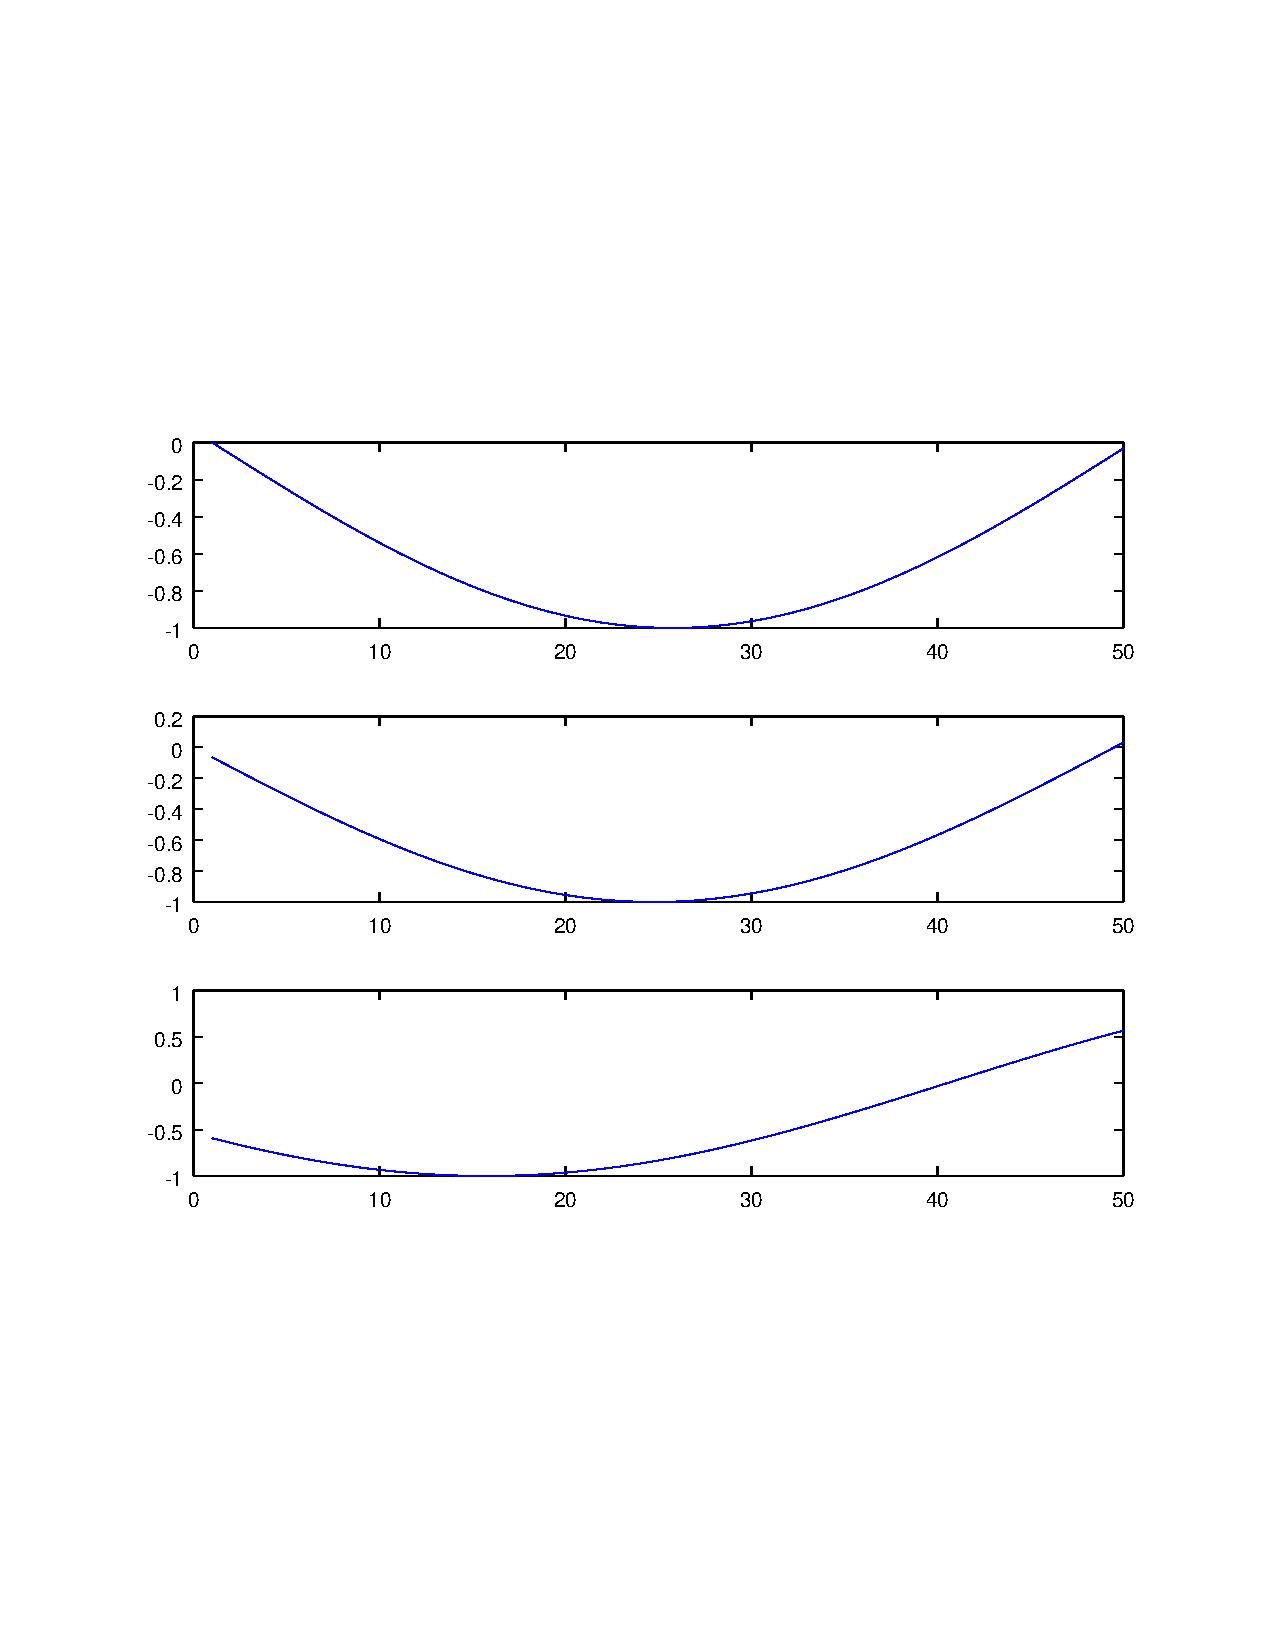
\includegraphics[scale=0.4]{Figures/lofreq}
%\caption{Different windows of the same signal}
%\label{fig:windowslo100}
%
%
%
%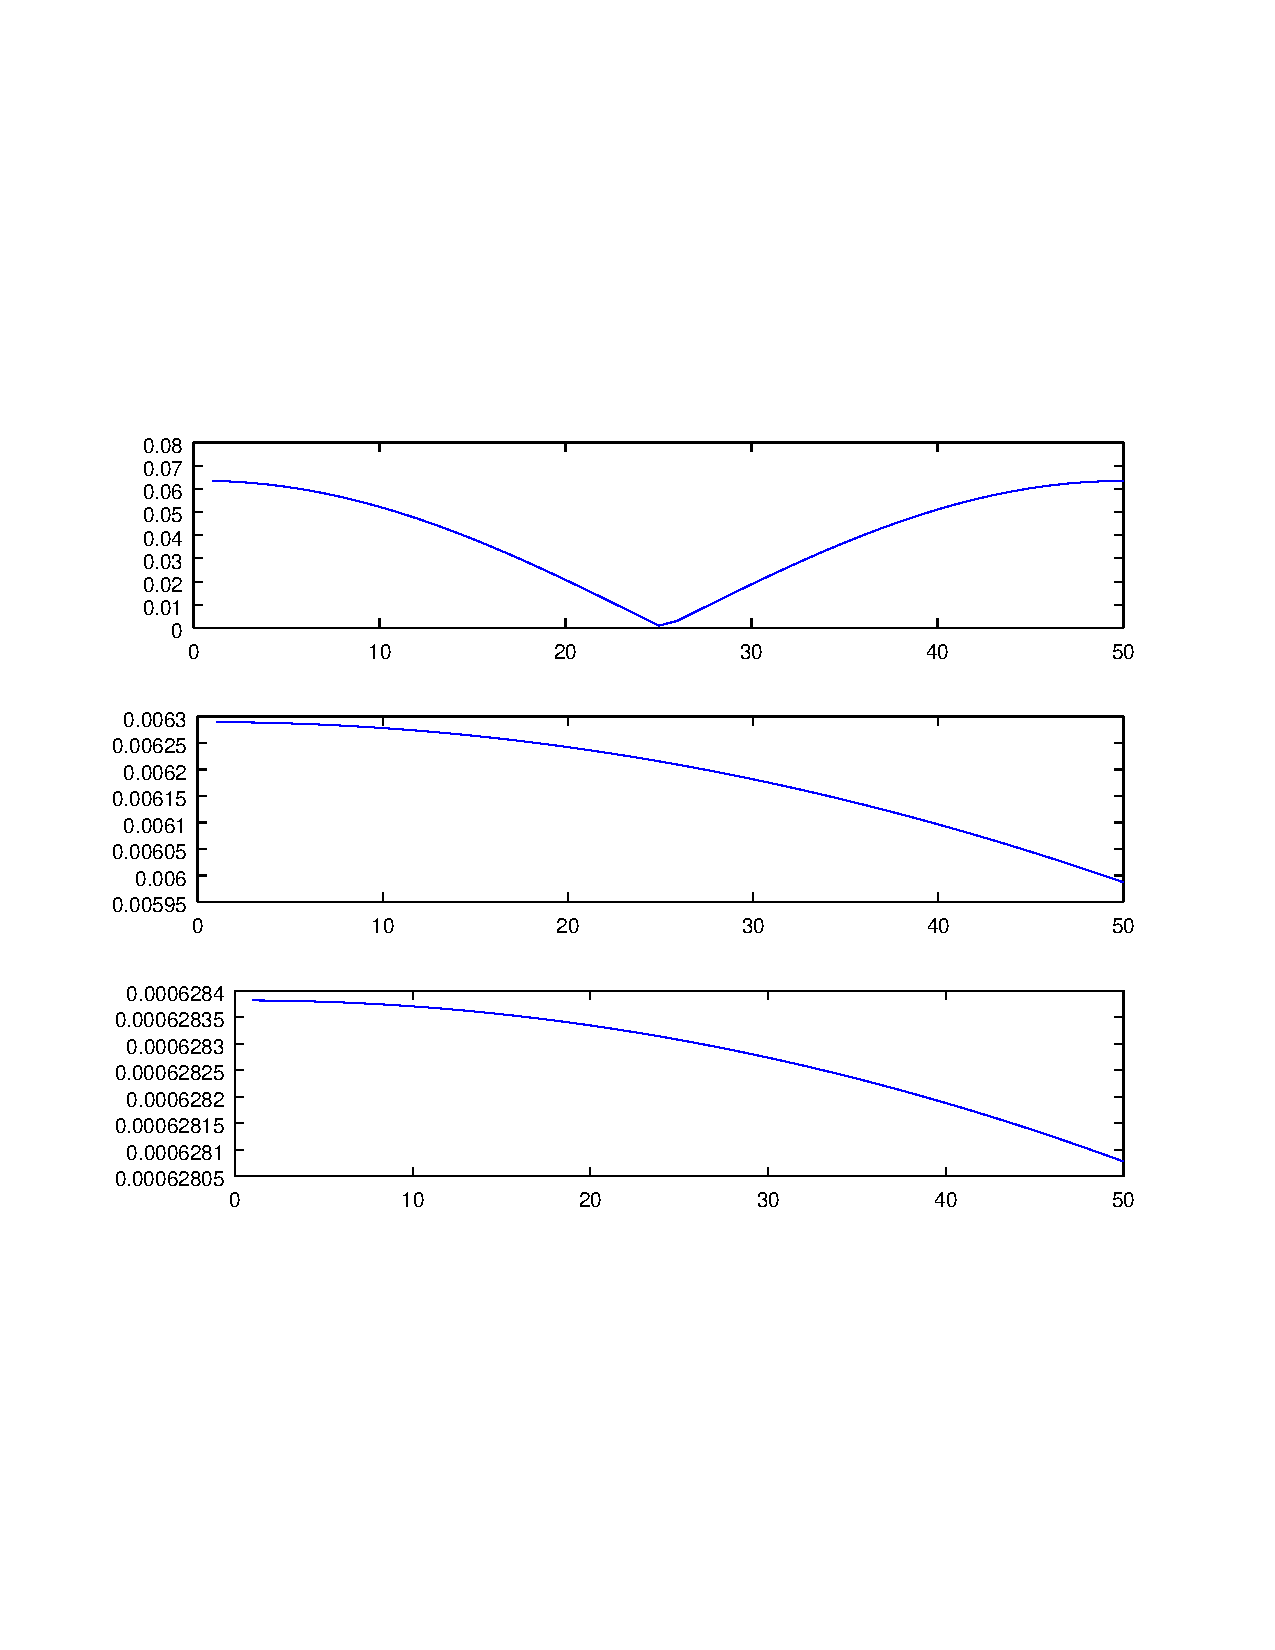
\includegraphics[scale=0.4]{Figures/absvals}
%\caption{Absolute differences between a signal and shifted counterpart, according to sample rate}
%\label{fig:absvals}
%\end{figure}
